\documentclass[12pt]{article}
\usepackage[utf8]{inputenc}
\usepackage[T2A]{fontenc}
\usepackage[english, russian]{babel}
\usepackage{amssymb}
\usepackage{amsmath}
\usepackage{ textcomp }
\textheight=250mm \textwidth=180mm \hoffset=-25mm \voffset=-30mm
%\textheight=55mm \textwidth=155mm \hoffset=-5mm \voffset=-7mm
%\usepackage{epsfig}
%\usepackage{graphicx}
%\usepackage{amssymb}
\pagestyle{empty}
\usepackage{graphicx}
\graphicspath{{/Users/admin/Desktop/}}
\graphicspath{{/}}
\DeclareGraphicsExtensions{.pdf,.png,.jpg}

\begin{document}
\begin{Large}
\begin{center}

\textbf{Техническое задание курсового проекта \\ "Судоку"\\}
\textit{Пьянков Семен, 572 группа\\
Вознюк Данила, 572 группа}

\end{center}
\end{Large}

\begin{enumerate}
\item \textbf{Цель проекта}\\
Целью курсового проекта является создание игры ''Судоку'' - с полями размера 9\texttimes9 и 16\texttimes16, user-friendly gui для этой игры.

    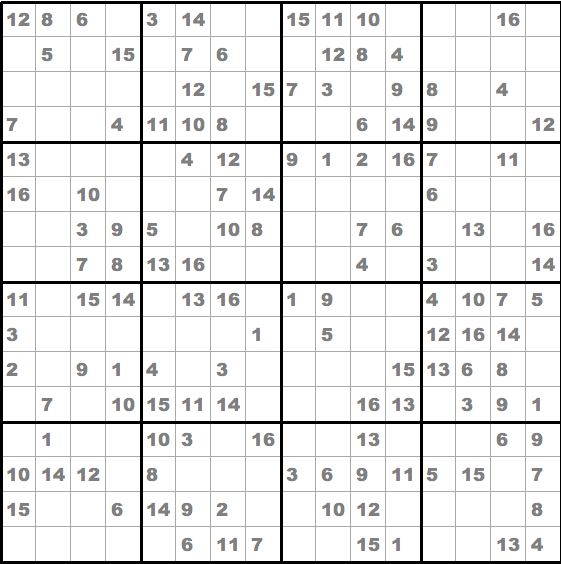
\includegraphics[width=10cm]{sixteen}
    
\item \textbf{Общая идея задачи}\\
В таблице 9\texttimes9 (16\texttimes16) должны быть расставлены числа от 1 до 9 (16) так, чтобы ни в одном столбце, строке и области 3\texttimes3 (4\texttimes4) (центральной, боковых и угловых) не было повторяющихся чисел (см. рисунок). Программа создает кроссворды разной сложности, по заполнении пользователем есть возможность проверить правильность заполнения.

    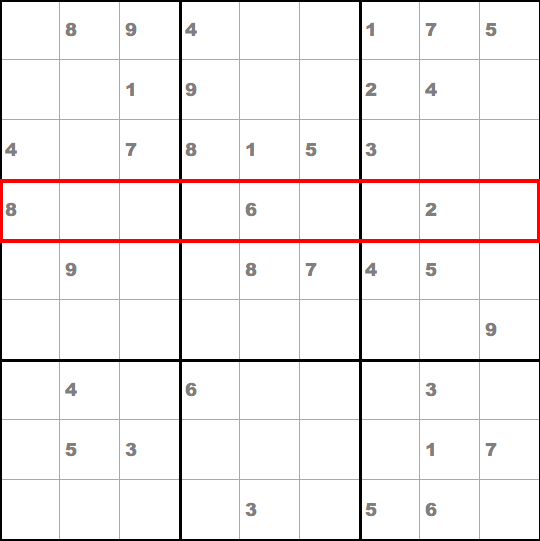
\includegraphics[width=5cm]{row}
    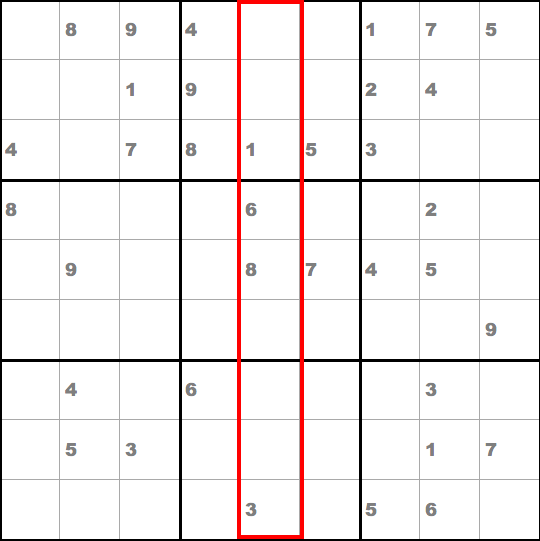
\includegraphics[width=5cm]{column}
    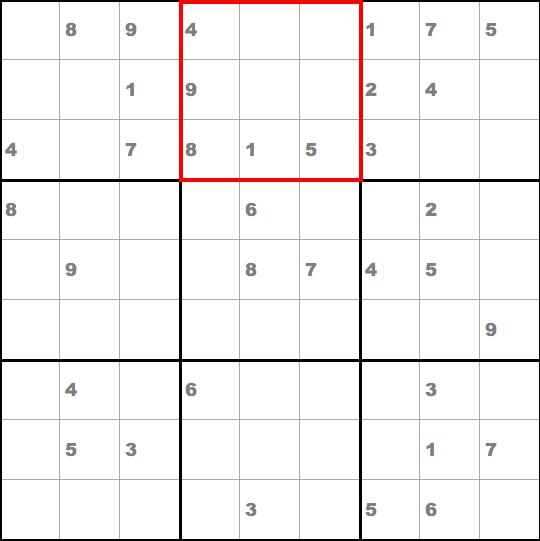
\includegraphics[width=5cm]{area}

\item \textbf{Основные подзадачи и их взаимосвязь}
\begin{itemize}
    \item Решение созданного судоку
    \item Создание заполненного поля из заранее заданного константного поля
    \item Создание кроссворда из заполненного поля
    \item Хранение решений в отдельной структуре
    \item Создание интерфейса приложения
\end{itemize}

\item \textbf{Общие предпосылки моделирования} \\
Модель судоку - двумерный массив, каждый элемент которого является набором возможных значений данной ячейки кроссворда. В отдельной модели хранится база решений судоку - очевидно, что для каждого кроссворда не должно быть больше одного уникального решения (отправная точка для генерации кроссворда). В начале используется sample - уже созданный решенный судоку (см. рисунок), элементы поля перемешиваются (не меняя правила кроссворда), выбирается случайное поле и удаляется. Это действие повторяется до тех пор, пока решений не станет больше одного.

    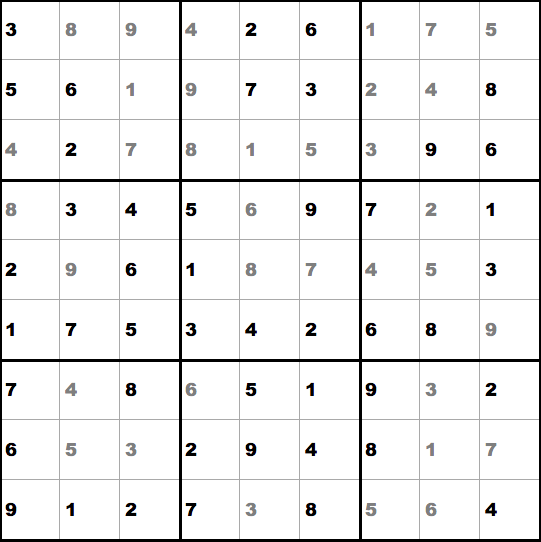
\includegraphics[width=7cm]{solved}
    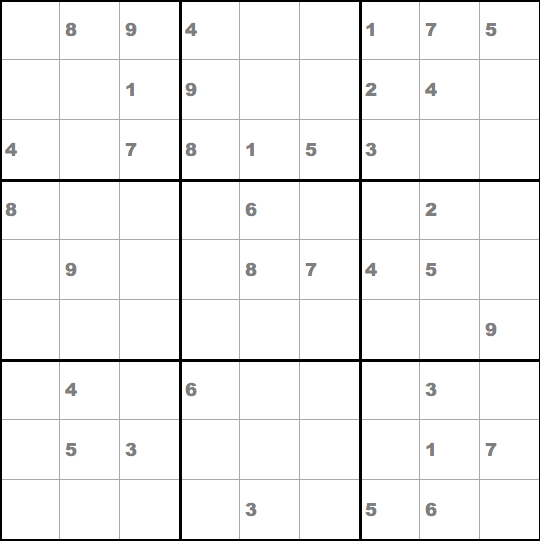
\includegraphics[width=7cm]{unsolved}

\item \textbf{Детальное описание содержания подзадач} \\
Заранее задан пример решенного судоку. Перемешиваем его, меняя местами отдельно строки и отдельно столбцы внутри каждой зоны 3\texttimes3 (4\texttimes4) и меняя местами два конкретных числа (например меняем местами все числа 2 и все числа 9).\\
Затем запускаем алгоритм генерации судоку из готового поля - он использует алгоритм решения кроссворда. В первую очередь заполняем для всех пустых элементов двумерного массива все возможные числа. Затем проверяем (исходя из правил судоку), какие числа не могут располагаться в каждой ячейке и удаляем их. Проверяем ячейки, в которых есть только одно возможное число, сохраняем его и повторяем эти проверки пока происходят изменения.\\
Если после этого все ячейки заполнены - все хорошо. Иначе делаем рекурсивный перебор с возвратом и находим все(!!!) решения.\\
Умея решать, начинаем генерировать поле судоку: из созданного и перемешанного поля удаляем по одному элементу и проверяем число решений после удаления. В случае сохранения единственности решения - сохраняем изменение, в обратном случае откатываем изменение. \textit{Возможность оптимизации - удаление сразу нескольких чисел или распараллеливание.}\\
Созданный массив выводится в интерфейс, написанный с использованием библиотеки Qt - из интерфейса есть возможность сохранять/загружать игры, решать судоку разной сложности, проверять на правильность решение, получать подсказки.\\

\item \textbf{Состав работ и исполнители} 
\begin{itemize}
    \item Ядро: структура кроссворда, алгоритм перемешки, алгоритм решения, алгоритм генерации судоку - \textit{Пьянков Семен, 572}
    \item Ядро: база решений, сохранение решений, оптимизация алгоритма генерации\\ - \textit{Вознюк Даниил, 572}
    \item Создание и отладка интерфейса - \textit{Совместная работа}
    \item \textbf{\textit{Дополнительно:}} возможность сохранения игр в виде исполняемых файлов - \textit{Вознюк Даниил, 572}
    \item \textbf{\textit{Дополнительно:}} создание кроссплатформенного приложения, способного запускаться под любой операционной системой вне зависимости от предустановленных библиотек - \textit{Пьянков Семен, 572}
\end{itemize}

\item \textbf{Используемые программные и технические средства} \\
Компилятор - clang, g++.\\
Операционные системы - MS Windows, Unix, macOS с установленной библиотекой Qt.

\end{enumerate}

\end{document}